\section{approach}
\label{sec:approach}
In this section, we first formulate the just-in-time defect prediction and provide an overview of our framework. We then describe the details of each part inside the framework. Finally, we present an algorithm for learning effective settings of our model's parameters. 
\subsection{Framework Overview}
\label{sec:overview}

\begin{figure}
\center
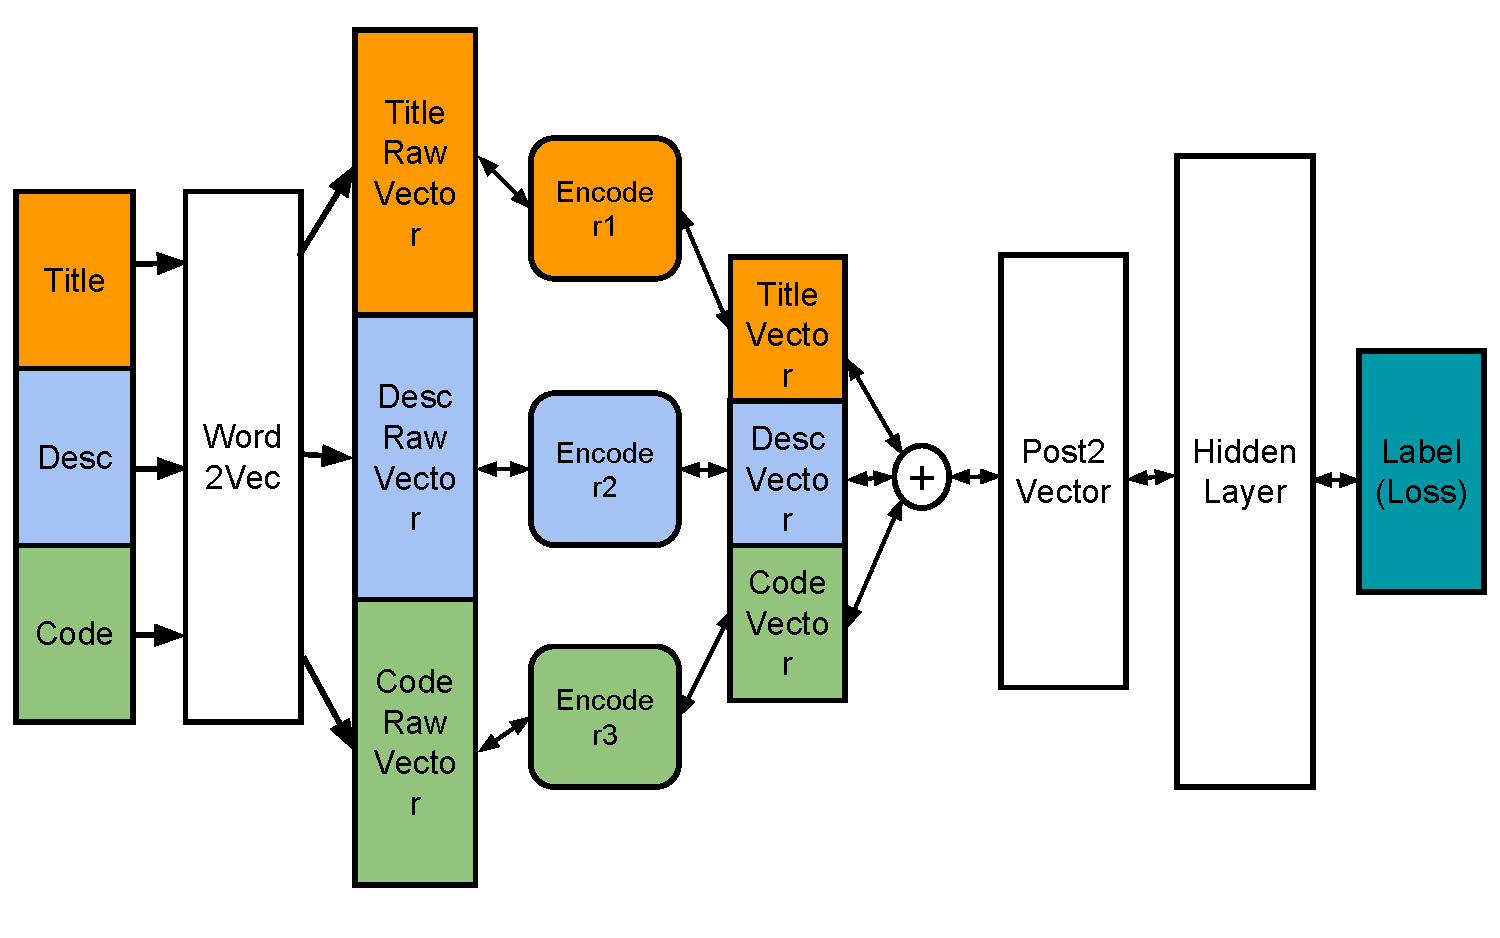
\includegraphics[scale=0.36]{figs/framework.pdf}
\caption{The general framework of just-in-time defect prediction model.}
\label{fig:overview}
\end{figure}

The goal of the just-in-time defect prediction model is to automatically label a commit change as bug or clean to help developers better focus on their efforts on assuring software quality. We consider the just-in-time defect prediction problem as a learning task to construct prediction function: $f:
\mathcal{X} \longmapsto \mathcal{Y}$, where $y_i \in \mathcal{Y} = \{0, 1\}$ indicates whether a commit change $x_i \in \mathcal{X}$ cleans ($y_i = 0$) or contains a buggy code ($y_i = 1$). The prediction function $f$ can be learned by minimizing the following objective function:
\begin{equation}
\underset{f}{min} \sum_{i}\mathcal{L}(f(x_i), y_i) + \lambda\Omega(f)
\end{equation}
where $\mathcal{L}(.)$ is the empirical loss function measuring the difference between the predicted and the output label, $\Omega(f)$ is a regularization function to prevent the over fitting problem, and $\lambda$ the trade-off between $\mathcal{L}(.)$ and $\Omega(f)$. Figure~\ref{fig:overview} illustrates the overview framework of the just-in-time defect prediction model. The model consists of four parts: input layer, feature extraction layer, feature combination layer, and the output layer. We explain the details of each part in the following subsections.

\subsection{Input Layer}
\label{sec:input_layer}
To feed the raw textual data to convolutional layers for feature learning, we first encode a commit message and code changes in the input layer. We represent each word in the commit message and code changes as $d$-dimensional vector. After the preprocessing step, the $\mathcal{X}^{m}_i$ and $\mathcal{X}^{c}_i$, which are the encoded data of the commit message and code changes respectively, are passed to the convolutional layers to extract the commit message and code changes features. In the convolutional layers, the commit messages and code changes are processed independently to extract the features based on each type of textual information. These features from the commit messages and code changes are then combined into a unified feature representation, and followed by a linear hidden layer connected to output layer used to produce the output label $\mathcal{Y}$ indicating whether the commit change $x_i$ cleans or contains a buggy code. 

The novelty of the just-in-time defect prediction model lies in the convolutional network layers for code changes and the feature combination layers. In the following subsection, we firstly discuss the convolutional layers for the commit message and present the novelty of our model in more details. 

\subsection{Convolutional Network Architecture for Commit Message}
\label{sec:cnn_message}